\documentclass{report}
\usepackage[utf8]{inputenc}
\usepackage{lib/report-template}
\usepackage[all]{background}
\usepackage{lipsum}

\usepackage{titlesec}
\titleformat{\chapter}
  {\normalfont\LARGE\bfseries}{\thechapter}{1em}{}
\titlespacing*{\chapter}{0pt}{3.5ex plus 1ex minus .2ex}{2.3ex plus .2ex}

\SetBgContents{Preliminary version/1.0}% Set contents
\SetBgPosition{-0.5cm,-5.0cm}% Select location
\SetBgOpacity{1.0}% Select opacity
\SetBgAngle{90.0}% Select rotation of logo
\SetBgScale{2.0}% Select scale factor of logo


%Line spacing
\renewcommand{\baselinestretch}{1.5}

\title{projeto ATLAS}

\date{August 2019}


\begin{document}

\begin{titlepage}.
    \begin{tikzpicture}[remember picture,overlay]

% UTT Background under the title and info box
\coordinate [right=8mm, below=70mm] (uttbackground_anchor) at (current page.north west);
\node [name=uttsquare,anchor=north west] at (uttbackground_anchor){
%\includegraphics[width=19.4cm]{first-page-background.png}};
%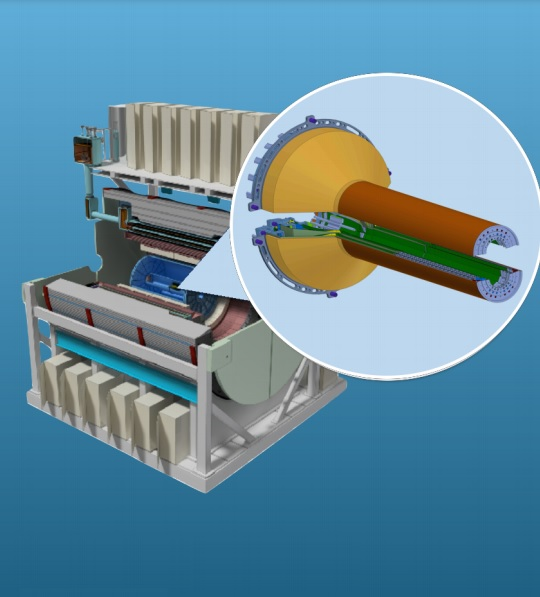
\includegraphics[width=19.4cm]{assets/sPhenix_front.JPG}};
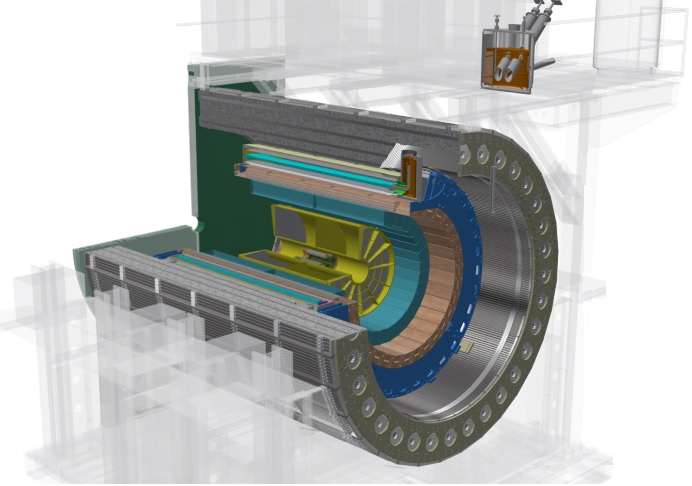
\includegraphics[width=19.4cm]{assets/mvtx_front.jpg}};

\end{tikzpicture}

    % Margin to begin the text under the uttsquare
    \vspace{3.5cm}

    % Internship title
    
    \begin{textblock*}{15cm}(3cm,2cm)
        \begin{Huge}
            \begin{center}
                \makeatletter
                \noindent\textcolor{black}{ Projeto de pesquisa de pós-doutorado em física}
                \makeatother
            \end{center}
        \end{Huge}
    \end{textblock*}
    
    % project tipe
    \begin{textblock*}{15cm}(2.5cm,5.5cm)
        \makeatletter
        \begin{LARGE}
            \begin{center}
                \color{black}
                {\it  }\\
            \end{center}
         \end{LARGE}
     
    \end{textblock*}
    
    %TITLE
    \begin{textblock*}{17.5cm}(2cm,5cm)
        \begin{Huge}
            \begin{center}
                \makeatletter
                \noindent\textcolor{white}{\textbf{Desenvolvimento de um detector de silício para a medida de vértice no experimento sPhenix}}
                \makeatother
            \end{center}
        \end{Huge}
    \end{textblock*}

    % Author
    \begin{textblock*}{15cm}(2.5cm,23cm)
        \begin{LARGE}
        \begin{center}
            \color{white}
                \textbf{Autor :} Dr. Renato Aparecido Negrão de Oliveira 
        \end{center}
            
        \end{LARGE}
        
    \end{textblock*}
    
    % FOOT NOTE
    \begin{textblock*}{15cm}(3cm,25cm)
        \makeatletter
        \begin{center}
            {\color{white}
                \textbf{SÃO PAULO, 2020} 
            }
        \end{center}
        \makeatother
    \end{textblock*}

\end{titlepage}

%\begin{titlepage}.
    \begin{tikzpicture}[remember picture,overlay]

% UTT Background under the title and info box
\coordinate [right=8mm, below=70mm] (uttbackground_anchor) at (current page.north west);
\node [name=uttsquare,anchor=north west] at (uttbackground_anchor){
%\includegraphics[width=19.4cm]{first-page-background.png}};
%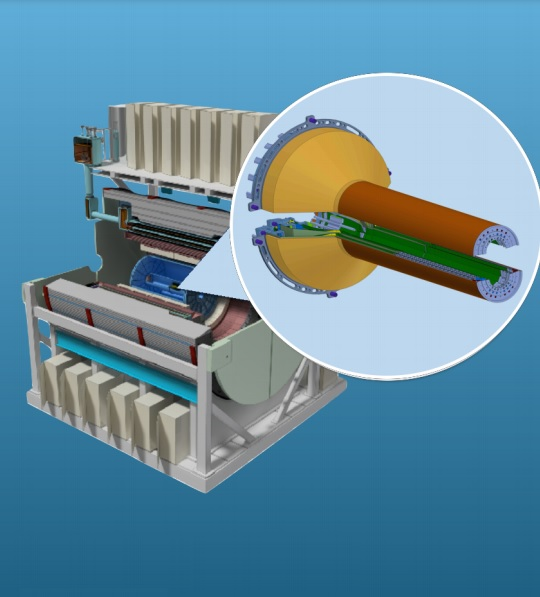
\includegraphics[width=19.4cm]{assets/sPhenix_front.JPG}};
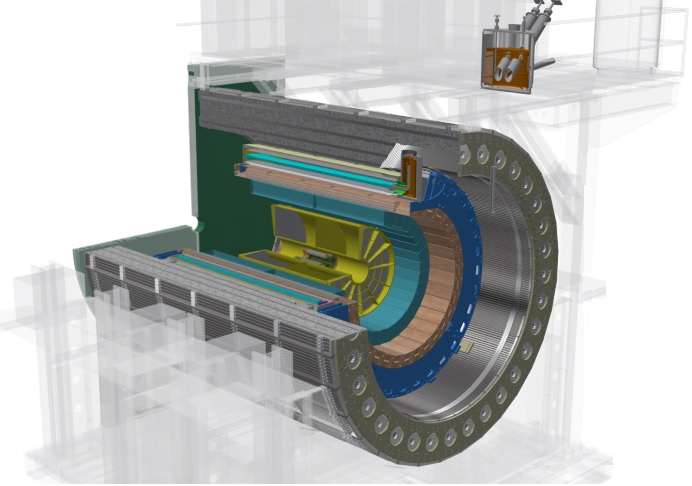
\includegraphics[width=19.4cm]{assets/mvtx_front.jpg}};

\end{tikzpicture}

    % Margin to begin the text under the uttsquare
    \vspace{3.5cm}

    
    % Authhor
    \begin{textblock*}{15cm}(3cm,2.cm)
        \makeatletter
        \begin{huge}
            \begin{center}
                \color{black}
                 Renato Aparecido Negrão de Oliveira\\ 
            \end{center}
         \end{huge}
     
    \end{textblock*}
    
    %TITLE
    \begin{textblock*}{15cm}(3cm,12cm)
        \begin{Huge}
            \begin{center}
                \makeatletter
                \noindent\textcolor{white}{Desenvolvimento de um detector de silício para a medida de trajetórias e tempo no experimento ATLAS-LHC}
                \makeatother
            \end{center}
        \end{Huge}
    \end{textblock*}

    % Info box
    \begin{textblock*}{15cm}(2.5cm,20cm)
        \makeatletter
        \begin{LARGE}
            \setcellgapes{4pt}
            \makegapedcells
            {\color{black}\begin{tabularx}{15cm}{XX}
                \textbf{Supervisor :} Dr. Marco Aurélio Lisboa Leite (IFUSP)\\ 
                %\textbf{Supervisor :} Dr. Marcelo Gameiro Munhoz (IFUSP)
            \end{tabularx}}
        \end{LARGE}
        \makeatother
    \end{textblock*}
    
    % FOOT NOTE
    \begin{textblock*}{15cm}(3cm,24cm)
        \makeatletter
        \begin{center}
            {\color{black}
                \textbf{SÃO, PAULO 2020} 
            }
        \end{center}
        \makeatother
    \end{textblock*}

\end{titlepage}


\chapter*{Resumo}

O experimento sPHENIX, atualmente em fase de desenvolvimento, é um experimento científicos de ultima geração dedicado ao estudo das propriedades do plasma de quarks e gluons (QGP). Esse experimento será construído no Relativistic Heavy Ion Collider (RHIC) no Brookhaven National Laboratory (BNL). 

Para atender às demandas experimentais, o sPHENIX  MASP-based Vertex Detector (MVTX) permitirá reconstruir os eventos à uma alta taxa de colisão utilizando sensores finos com baixa quantidade de material. Esse sistema de detecção irá fornecer uma alta eficiência na reconstrução de trajetórias e uma excelente resolução na medida do parâmetro de impacto, características ideais para identificar hádrons oriundos de quarks pesados, e reconstrução de eventos para as altas taxas de colisão que serão fornecidas pelo RHIC.

A vista disso, neste documento é proposto o desenvolvimento de atividades de pesquisa em colaboração com o experimento sPHENIX. O trabalho será focado na pesquisa e desenvolvimento dos sensores semicondutores do tipo MAPS - recentemente desenvolvidos para tolerar altos níveis de radiação ionizante - com o objetivo de optimizar sua capacidade para utilização no detector MVTX do experimento sPHENIX.


\chapter*{Abstract}

The sPHENIX experiment is a next-generation high energy nuclear physics experiment, currently under development for the Relativistic Heavy Ion Collider (RHIC) at Brookhaven National Laboratory (BNL). It is designed to study the nature of the QGP by measuring fully reconstructed jets  at higher collision rates. 

To meet the experimental demands, the sPHENIX  MASP-based Vertex Detector (MVTX) will provide fast counting rates and a very low material budget with pixel sensors. This detector will enable a high tracking efficiency and excellent impact parameter resolution, ideal for heavy flavor hadron identification and reconstruction at the very high beam collision rates provided by RHIC.

Therefore, in this document, it is proposed to be performed activities on research and development in collaboration with sPHENIX experiment. The research will be focused on the development of the MAPS sensors - recently developed to operate at higher levels of radiation dose - to optimize the device capabilities to operate in the sPHENIX MVTX detector.



\tableofcontents

\chapter{Introdução}

O experimento sPHENIX, atualmente em fase de desenvolvimento, se constitui em um experimento científico de ultima geração, dedicado ao estudo das propriedades do plasma de quarks e gluons (QGP). Esse experimento será construído no Relativistic Heavy Ion Collider (RHIC) no Brookhaven National Laboratory (BNL), e está programado para entrar em operação no ano de 2023.

O sPHENIX foi desenhado empregando as mais recentes e eficientes técnicas experimentais existentes para a detecção de partículas, com o objetivo de estudar a natureza da interação forte de quarks pesados com o plasma de quarks e gluon (QGP). 

Neste sentido, grandezas como o fator de modificação nuclear e o fluxo elíptico V$_{2}$ de quarks pesados são observáveis importantes que somados à reconstrução de jatos oriundos de quarks pesados, charm e bottom, oferecem informações fundamentais para o entendimento das propriedades dos QGP, tornando possível estudar a perda de energia desses partons no meio em função da massa dos quarks e temperatura do plasma.

Do ponto de vista experimental, a medida desses observáveis requer alta precisão e eficiência na reconstrução das trajetórias próximas ao ponto de interação, de modo a fornecer uma identificação precisa dos vértices secundários oriundos de quarks pesados. Assim, um detector de vértice com alta velocidade e grande aceitação torna-se necessário para medir esses observáveis.  

Para contornar esse desafio experimental, o sPHENIX irá construir um detector de vértice composto por detectores de silício pixelados, cujos sensores empregarão a tecnologia denominada Monolithic Active Pixel Sensor (MAPS), utilizada em diversos experimentos com altas taxas de colisão. O detector proposto, denominado MASP-based Vertex Detector (MTVX), utilizará sensores MAPS de ultima geração garantindo que o sistema tenha alta performance e seja capaz de efetuar as medidas em rapidez central e altas taxas de colisão, para um grande intervalo de momento transversal.

Possuindo excelentes características , o MVTX irá possibilitar o estudo da física de quarks pesados \textit{c} e \textit{b} no QGP, para as energias disponíveis no RHIC. Esses estudos estão além da capacidade de medida dos experimentos atuais presentes no RHIC, sendo desse modo importantes para o entendimento das propriedades de transporte no QGP nas energias do RHIC.

O detector MVTX fornecerá uma alta taxa de contagem utilizando sensores finos com baixa quantidade de material e espessura de $30\mu m$. Esse sistema de detecção irá fornecer uma alta eficiência na reconstrução de trajetórias e uma excelente resolução na medida do parâmetro de impacto, características ideais para identificar hádrons oriundos de quarks pesados, e reconstrução de eventos para as altas taxas de colisão que serão fornecidas pelo RHIC.

%2 proposta do projeto
A vista disso, o propósito deste projeto é desenvolver técnicas e metodologias necessárias para a caracterização física de sensores semicondutores do tipo MAPS, e dos componentes do detector MVTX. Neste escopo a colaboração com o experimento sPHENIX será fundamental pois irá servir de ponte para o intercambio de conhecimento e experiência que serão importantes, permitindo introduzir futuramente esse tipo de tecnologia no Brasil.

O projeto será composto de várias etapas onde inicialmente pretende-se consolidar as técnicas necessárias para a caracterização dos sensores e montagem do detector. Neste processo o pesquisador e colaboradores irão estabelecer os 
métodos experimentais para a caracterização das propriedades físicas dos sensores. Nesta estágio, o pesquisador será responsável por montar e certificar os arranjos experimentais, desenhar e construir as partes necessárias para os mesmos, além de automatizar o processo de tomada de dados. Por fim, a discussão dos resultados obtidos com os centros de pesquisa dentro da colaboração sPHENIX será feita para garantir a qualidade dos resultados obtidos e acelerar sua consolidação.

Neste ponto é importante destacar que a implantação dessa linha de pesquisa no grupo HEPIC do Instituto de Física da Universidade de São Paulo será importante para projetos futuros envolvendo sensores semicondutores. Atualmente o grupo conta com ferramentas na área de instrumentação para física nuclear e de partículas reconhecida internacionalmente, e adquirida por meio da execução de projetos em colaborações internacionais, como por exemplo o chip SAMPA focada na tecnologia de detectores gasosos \cite{ref1}. Isso somado à experiência do pesquisador responsável adquirida na execução de pesquisa e desenvolvimento no âmbito do projeto de upgrade do TPC do ALICE \cite{tpcNIM,discharge_paper,GSI_REPO}, tornará possível a transferência total de tecnologia relacionada com sensores semicondutores de alta performance para o HEPIC, bem como a geração de novas tecnologias e aplicações.

\renewcommand{\cleardoublepage}{}
\renewcommand{\clearpage}{}
\chapter{O detector de vértice MVTX}

O MVTX do experimento sPHENIX é um detector extremamente sofisticado dedicado a medida da posição do vértice do evento, e que foi desenhado empregando os últimos avanços tecnológicos desenvolvidos para esse tipo de detector \cite{1}. A Fig. \ref{mvtx} mostra em detalhes a vista transversal do experimento sPHENIX, próxima à linha do feixe, e a localização do detector MVTX juntamente com outros sistemas de detecção, TPC, INTT, EMCal e inner/outer HCAl \cite{1}, os quais empregam outras técnicas de medida.

Os principais requisitos considerados durante o processo de 
desenvolvimento do detector para garantir a ótima resolução na identificação dos vértices primário e secundários, alta eficiência na reconstrução de trajetórias, e alta taxa de aquisição são listados a seguir:

\begin{itemize}
 
\item Para garantir a qualidade na identificação da posição do vértice a distância entre as primeiras camadas do detector e a linha do feixe foi reduzida ao mínimo.

\item Utilização de sensores de silício finos, reduzindo a quantidade de material utilizado e subsequentemente o espalhamento múltiplo das partículas no material, o que por fim reduz o fundo produzido no experimento. Essa medida é importante pois melhora a resolução na medida da multiplicidade do evento.

\item A segmentação do detector é importante para determina a qualidade na reconstrução das trajetórias, desse modo uma segmentação fina das camadas do MVTX foi adotada.

\item Baixo tempo de integração do sinal, para minimizar o pile-up de eventos, mantendo a ocupação do detector baixa, permitindo a sua operação no valor nominal de 200kHz em colisões Au+Au, e 13MHz para colisões p+p. 

\end{itemize}

Considerando todos esses requisitos, o MVTX será constituído utilizando três camadas de sensores de silício composto por pixel. O volume sensível do dispositivo será construído com uma camada de silício de alta resistividade acoplada a uma matriz de diodos coletores de cargas, formando cada pixel do sensor, e a eletrônica responsável por amplificar e digitalizar o sinal. A leitura de cada pixel será feita individualmente durante a aquisição de dados.       

\begin{figure} 
    \centering
    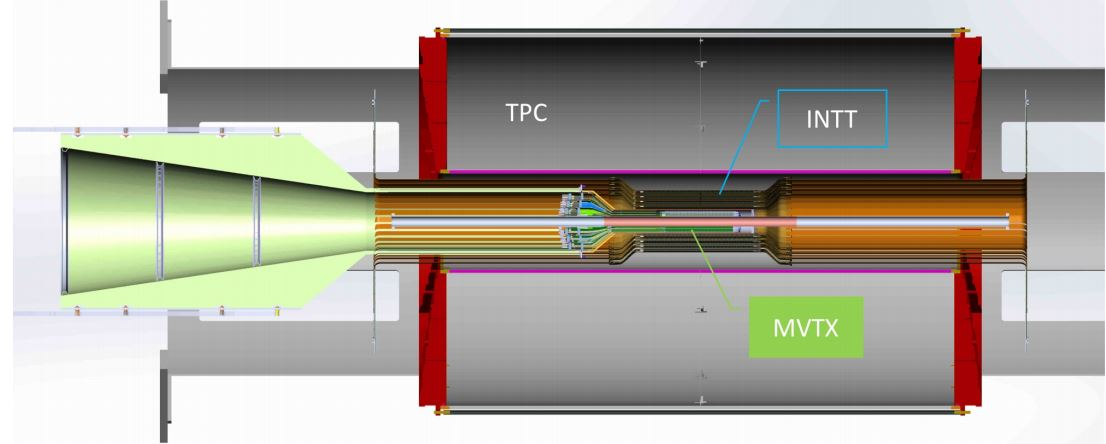
\includegraphics[width=16cm]{assets/mvtx.JPG}
    \caption{ Figura mostrando no detalhe a posição onde o MVTX será instalado. A figura também mostra o experimento sPHENIX e os seus vários sistemas.}
    \label{mvtx}
\end{figure}

%%%mechanica do detector
Como mostra a Fig. \ref{mvtxdetail}.a, cada suporte do MVTX, denominado \textit{stave}, será instrumentalizado com uma fileira de chips com pixelados, que serão colados na placa de refrigeração, e conectados ao circuíto impresso flexível de leitura dos sinais por meio de uma solda de ligação. Como mostra a Fig. \ref{mvtxdetail}.b uma conexão mecânica permitirá que o suporte com os chips sejam conectados ao \textit{end wheel} de onde uma extensão do circuito flexível segue para o \textit{patch panel}, Fig. \ref{mvtxdetail}.c, onde as conexões elétricas são feitas, e onde estão localizados também os serviços de refrigeração e alimentação de baixa tensão dos sensores.

\begin{figure} 
    \centering
    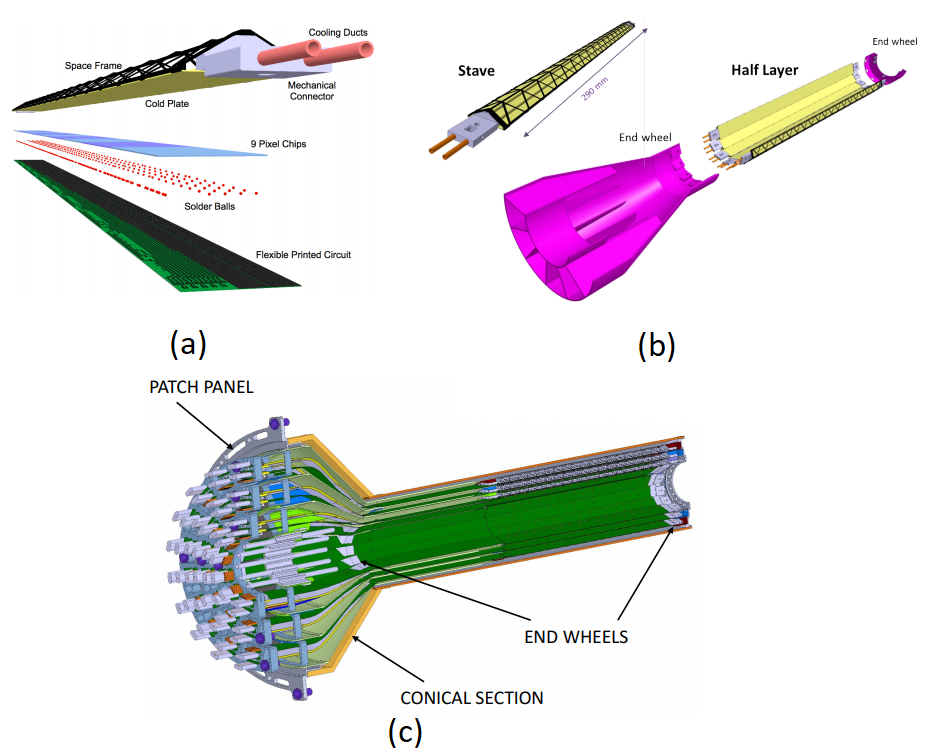
\includegraphics[width=16.0cm]{assets/mvtx_detail.JPG}
    \caption{Figura mostrando detalhes do detector MVTX: (a) Vista esquemática de uma \textit{stave} do MVTX. (b) MVTX \textit{stave}, e conjunto de \textit{staves} fixadas em um suporte formando metade de um barril do detector. (c) Vista da metade do detector MVTX montado com três camadas fixadas no \textit{end wheel}.}
    \label{mvtxdetail}
\end{figure}

\renewcommand{\cleardoublepage}{}
\renewcommand{\clearpage}{}
% Conteúdo do capitulo 
% 1- Desenvolver e caracterizar sensores MAPS para o upgrade do ATLAS
%2- Estudar experimentalmente os processos físicos relacionados com a amplificação da carga
%3- Melhorar os sensor por intermédio de simulações comparando com dados experimentais
%4- Desenvolvimento de um sistema de aquisição
%5- perspectivas de outros trabalhos
\chapter{Objetivos do projeto}

% 1- Desenvolver e caracterizar sensores LGAD para o upgrade do ATLAS
O objetivo deste projeto é caracterizar e desenvolver sensores semicondutores do tipo MAPS para o experimento sPhenix, bem como para outras aplicações no âmbito do Instituto de Física da USP. O trabalho será dividido em fases as quais visam em um primeiro momento consolidar o {\it know how} sobre essa tecnologia, e em um segundo momento, com as competências consolidadas, contribuir para a melhoria do sensor e suas aplicações em diversas áreas da ciência, bem como para o sPHENIX.

Como exposto anteriormente, no contexto da colaboração sPHENIX, o pesquisador responsável participará ativamente na qualificação dos sensores e na consolidação de suas especificações. Em seguida, uma vez definidos os sensores, os mesmos serão produzidos em larga escala, e neste ponto o grupo fará parte do esforço em conjunto com o experimento sPHENIX para qualificar os MASP que serão empregados na construção do MVTX. Esse trabalho será fundamental para o exercício dos métodos experimentais a serem desenvolvidos.

%2- Estudar experimentalmente os processos físicos relacionados com a amplificação da carga
Em seguida, com a implantação das diversas metodologias experimentais para a caracterização dos sensores semicondutores será possível estudar em grande detalhe os processos físicos relacionados com a amplificação de carga e a produção de sinal no material semicondutor, visando compreender e melhorar os processos de fabricação baseando-se no aumento do ganho, resolução temporal e estabilidade elétrica dos sensores durante sua operação em ambiente com alta radiação \cite{}. 

Como resultado espera-se produzir novas gerações de sensores os quais poderão ser utilizados não apenas para a detecção de partículas carregadas, mas como detector de raios-X. Devido às excelentes características dos detectores do tipo MAPS, as quais incluem sua alta eficiência quântica para uma grande faixa de comprimentos de onda e a possibilidade de construir detectores com alta granularidade, aplicações em diversos ramos envolvendo a detecção de raios-X, tais como luz síncrotron, tornam-se muito atrativas e de fácil implantação uma vez estabelecida essa tecnologia.

%3- Melhorar os sensor por intermédio de simulações comparando com dados experimentais
Outro aspecto importante que também será trabalhado neste projeto é o estudo de melhorias na geometria do MAPS por intermédio de simulações e modelos computacionais, e a comparação direta com dados experimentais medidos em laboratório para a validação do modelo. Esse trabalho será fundamental para possibilitar a melhoria do sensor, além de produzir um modelo validado capaz de fazer predições para o caso de novos designs de sensores semicondutores. 

%4- Desenvolvimento de um sistema de aquisição
Além do desenvolvimento dos sensores MAPS, um outro objetivo deste projeto será o de integrá-lo a um sistema de aquisição de dados, o que tornará possível a reconstrução de eventos. Como resultado espera-se desenvolver todas as competência e habilidades presentes nos diversos componentes que compõem o sistema de aquisição, desde os aspectos físicos relacionados com a produção do sinal até o tratamento dos dados produzidos.

%5- perspectivas de outros trabalhos
Por fim, o desenvolvimento de algorítimos para a reconstrução dos eventos do experimento sPHENIX utilizando o MVTX não serão inclusos de início como objetivos neste projeto, no entanto tendo em vista a importância deste componente para o desenvolvimento do sistema de detecção e aquisição o mesmo poderá, como uma perspectiva futura, ser trabalhado mais adiante no projeto. 


\renewcommand{\cleardoublepage}{}
\renewcommand{\clearpage}{}
% Conteúdo do capitulo
%1 - Descrição do desafio experimental para o sphenix
%2 - Desafio de estabelecer o setup experimental
%3 - Desafio de melhorar o sensor LGAD
%4 - Desafio de aplicar para a medida de raios-x
%5 Considerações finais
\chapter{Desafios científicos e tecnológicos}

% 1 - Descrição do desafio experimental para o 
Como descrito anteriormente no texto desta proposta, o desafio científico deste projeto é desenvolver um detector semicondutor para a região de pseudo-rapidez central que seja capaz de melhorar a precisão na medida e na reconstrução de partículas ionizantes no ambiente de operação do experimento sPHENIX. 

Para superar esse desafio científico, este projeto irá trabalhar na pesquisa e desenvolvimento do sistema de detecção MVTX, cuja a técnica experimental é baseada na medida do sinal produzido com a energia depositada pelas partículas nos pixel que compõem o detector, tornando dessa forma possível associar as partículas ao seu vértice de produção para colisões Ouro-Ouro no RHIC. Para realizar a construção do MVTX, os sensores do tipo MAPS serão adotados como base tecnológica, tendo em vista que eles apresentam excelentes características com respeito ao ganho em altas taxas de colisão. 

% FASE 1
%2 - Desafio de estabelecer o setup experimental
A fase inicial do projeto terá como foco o desenvolvimento da metodologia experimental necessária para a caracterização dos sensores MAPS. Isso será feito através da implantação de técnicas  com o objetivo de caracterizar os sensores MAPS em termos de sua corrente de fuga, ganho, uniformidade e resolução temporal.

Com as técnicas experimentais estabelecidas para a medida da:

\begin{itemize}
\item Corrente de fuga
\item Ganho e uniformidade do ganho
\item Resolução temporal 
\end{itemize}
será possível diagnosticar com precisão a qualidade dos sensores MAPS.

%3 - Desafio de melhorar o sensor LGAD
Uma vez consolidada os experimentos descritos acima para a caracterização dos sensores MAPS, o passo seguinte será continuar com o desenvolvimento do dispositivo, e com base nos dados coletados buscar discutir e optimizar os parâmetros do sensor com o objetivo de produzir novas gerações de MAPS com melhores características em termos de ganho, resolução temporal, uniformidade e resistência à radiação. 

Como dito anteriormente, o programa de pesquisa proposto neste projeto será em grande parte baseado na interação com a colaboração sPHENIX, de modo que teremos acesso aos recentes avanços obtidos no desenvolvimento do MASP, tais como a identificação de vulnerabilidades presentes na geometria do sensor e a degradação do material semicondutor devido ao dano radioativo, os quais serão também tópicos para investigação neste projeto.

Com a diminuição do ganho devido ao dano radioativo, ocorre um aumento da corrente consumida pelo dispositivo MAPS, o que por sua vez provoca o aumento na potência dissipada. Esse fator influencia o projeto de vários outros componentes que farão parte do detector para que seja possível dimensioná-los de forma adequada para comportar a carga de calor produzida pelo dispositivo. Estas questões  demonstram a grande importância de um estudo detalhado desses aspectos durante a fase de pesquisa e desenvolvimento do sensor. 

O design do MVTX encontra-se em seu estágio inicial de desenvolvimento, e desse modo inúmeras oportunidades para contribuição intelectual estão em aberto para serem exploradas na próxima fase da pesquisa e desenvolvimento que está para ser iniciada. 

% CONSIDERACOES FINAIS

Por fim, esta proposta de projeto tem como objetivos estratégicos de curto prazo preparar os experimentos necessários para o desenvolvimento do MAPS, e por conseguinte colaborar com o experimento sPHENIX na construção do MVTX. E para médio e longo prazo os objetivos de desenvolver dispositivos semicondutores para diversas aplicações científicas no âmbito nacional e internacional, e com isso consolidar a tecnologia para a fabricação de sensores semicondutores.

 %varios milestones estabelecidos

%Outro aspecto fundamental   

%Como descrito anteriormente, o ganho em um detector LGAD depende diretamente do perfil da concentração do dopante presente na camada de multiplicação do sensor. Dessa forma, o fator que mais contribui para o dano radioativo em sensores LGAD é a remoção e subsequente redução da concentração de dopante na camada de multiplicação o que por conseguinte provoca a redução do ganho e perdas na resolução em tempo. Com o R&D desenvolvido ate o momento, 

%preliminares demonstram que a adição de outros materiais, tais como carbono, junto com o material dopante podem minimizar o impacto do dano radioativo tornando os sensores mais resistentes à radiação ionizante, entretanto mais estudos devem ser conduzidos para compreender os fatores limitantes obtidos com a adição de outros materiais.


%incluindo a sua produção no Brasil. Vários pesquisadores que integram a equipe deste projeto vêm de outros grupos de pesquisa da USP, do IPEN, conferindo-lhe um forte carácter interdisciplinar, essencial no desenvolvimento de aplicações tanto em imagem de raios X, como na detecção de nêutrons.









\chapter{Cronograma de execução do projeto}

Como mostra a Fig. \ref{crono}, o plano de execução para o desenvolvimento do sPHENIX-MVTX tem a duração total de 3 anos (2020 - 2023), onde a produção dos dispositivos e a integração dos diversos componentes será executada. Neste contexto, como ilustra a seta em laranja na Fig. \ref{crono}, este projeto terá a duração inicial de um ano com início em 2021 e término em 2022, podendo claramente ser estendido de acordo com os compromissos assumidos durante esse período e a disponibilidade de recursos.
\\
\\
\begin{figure}[!h]
\centering
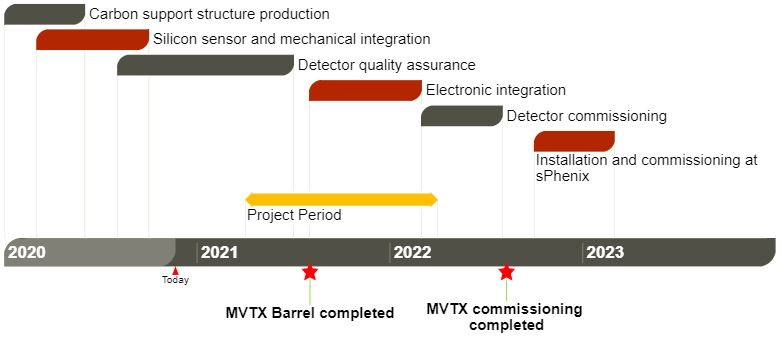
\includegraphics[width=15.0cm]{assets/cronograma.JPG}
\caption{Cronograma mostrando o planejamento para o desenvolvimento do MVTX. Os principais \textit{milestones} do projeto são mostrados em sua linha do tempo representados pelas estrelas em vermelho.}
\label{crono}
\end{figure}

Durante este período, o cronograma de desenvolvimento prevê o estabelecimento da infraestrutura para executar as medidas dos parâmetros de qualidade do sPHENIX-MVTX e sua integração com a eletrônica de aquisição de dados. Essas duas fases são importantes pois permitirá o desenvolvimento de atividades relacionadas com a caracterização do MVTX e seus diversos componentes, bem como a sua integração com o sistema de aquisição de dados, corroborando com os objetivos propostos neste documento. 

Por fim, os principais pontos do projeto de construção do sPHENIX-MVTX são mostrados em sua linha do tempo. De acordo com este cronograma, é importante destacar que o dispositivo estará completamente integrado em 2022.


\chapter{Disseminação e avaliação da pesquisa}

Uma vez que parte deste projeto está relacionada com aplicações à detecção de partículas, essa proposta possui um grande potencial de inovação tecnológica e poderá dar origem a diversos sensores, ampliando os direitos de propriedade intelectual dos processos e dispositivos produzidos na USP. Além disso, o pesquisador responsável possui experiência no desenvolvimento de instrumentação para física de altas energias, adquirida através do trabalho realizado no projeto de {\it upgrade} do TPC do experimento ALICE \cite{tpcNIM}, isso somado à infraestrutura presente no laboratório do HEPIC para o desenvolvimento de instrumentação nuclear, tornará possível estabelecer e consolidar a linha de pesquisa em sensores semicondutores no Departamento de Física Nuclear do Instituto de Física da USP. Isso irá corroborar com programas experimentais em andamento no grupo relacionado com a espectroscopia e reconstrução de imagens\cite{THGEM,NIM,xray}, ampliando a capacidade tecnológica do HEPIC com respeito à detecção de radiação ionizante. 

À vista disso, no âmbito nacional, com as ferramentas criadas será possível colaborar com os programas de instrumentação em diversos projetos de pesquisa presentes no Brasil tais como o Laboratório Nacional de Luz Síncrotron (LNLS), no que diz respeito ao desenvolvimento de sistemas de detecção. De acordo com os estudos levantados pelos pesquisadores do Sirius e descritas em seu projeto \cite{sirius}, {\it 'existe hoje no Brasil uma oportunidade excepcional para o desenvolvimento de expertise na área de detectores híbridos, visando atender às exigências das linhas de luz do Sirius. Futuramente, essa experiência poderá resultar em desenvolvimentos para as áreas médica, industrial e educacional'}. Isso está alinhado com os objetivos desta proposta.

No final do projeto, o {\it know how} adquirido estará consolidado e preparado para dar continuidade ao trabalho independente deste grupo em novas aplicações bem como na geração de novas tecnologias.

Finalmente, com relação ao gerenciamento do projeto, o seu andamento será monitorado por meio de reuniões semanais e apresentação de resultados ao grupo, onde será reunida as informações necessária para ajustar a estratégia de modo a cumprir os objetivos propostos. Por fim, no decorrer do projeto pretende-se produzir artigos técnicos e científicos documentando os avanços obtidos no desenvolvimento dos sensores, aumentando o impacto internacional do grupo de pesquisa e da tecnologia desenvolvida no Brasil.


\begin{thebibliography}{9}

\bibitem{sPHENIXproposal}A. Adare et al. \textit{An Upgrade Proposal from the PHENIX Collaboration}. arXiv:1501.06197, 2015.

\bibitem{1} sPHENIX Conceptual Design Report. 2017.

\bibitem{2} Jinrui Huang, Zhong-Bo Kang, and Ivan Vitev. \textit{Inclusive b-jet production in heavy ion collisions at the LHC}. Phys. Lett., B726:251–256, 2013.

\bibitem{3} S. S. Cao, G.Y. Qin, and S. A. Bass. \textit{Energy loss, hadronization and hadronic interactions of heavy flavors in relativistic heavy-ion collisions}. Phys. Rev., C92:024907, 2015.

\bibitem{4} Min He, Rainer J. Fries, and Ralf Rapp. \textit{Heavy-Quark Diffusion and Hadronization in Quark-Gluon Plasma}. Phys. Rev., C86:014903, 2012.

\bibitem{5} T. Song, H. Berrehrah, J. M. Torres-Rincon, L. Tolos, D. Cabrera, W. Cassing, and E. Bratkovskaya. \textit{Single electrons from heavy-flavor mesons in relativistic heavy-ion collisions}. Phys. Rev., C96:014905, 2017.

\bibitem{6} J.C. Xu, J.F. Liao, and M. Gyulassy. \textit{Bridging soft-hard transport properties of quark-gluon plasmas with cujet 3.0}. JHEP, 1602:169, 2016.

\bibitem{7}  L. Adamczyk et al. \textit{Measurement of D0 Azimuthal Anisotropy at Midrapidity in Au+Au Collisions at psNN=200GeV}. Phys. Rev. Lett., 118(21):212301, 2017.

\bibitem{8} G. Contin, L. Greiner, J. Schambach, M. Szelezniak, et al. \textit{The STAR MAPS-based PiXeL detector}. arXiv:1710.02176, 2017. 72.

\bibitem{9} B Abelev et al. \textit{Technical Design Report for the Upgrade of the ALICE Inner Tracking System}. J. Phys., G41:087002, 2014.

\bibitem{10} M. Mager. \textit{ALPIDE, the Monolithic Active Pixel Sensor for the ALICE ITS upgrade}. Nucl. Instrum. Meth., A824:434–438, 2016.

%%%%%%%%%%%%%%%%%%%%%%%%%%%%%%%%%%%%%%%%%%%%%%%%%%%%%%
\bibitem{ref1} B. A. et al. (ALICE Collaboration), Technical design report for the upgrade of the alice time projection chamber, CERN-LHCC-2013-020 A886 (2013), http://cds.cern.ch/record/1622286.


\bibitem{tpcNIM} M.M. Aggarwal, et al., Nucl. Instrum. Meth. A 903, (2018) 215–223. 

\bibitem{discharge_paper} A. Deisting, et al., Nucl. Instrum. Meth. A 937, (2019) 168–180.


\bibitem{GSI_REPO} Garabatos C., et al., Stability test of ALICE TPC GEM chambers at the LHC, GSI FAIR SCIENTIFIC REPORT 2017, DOI:10.15120/GSI-2017-01856.


\bibitem{THGEM} H. Natal da Luz, et al., EPJ Web of Conferences 174, (2018) 01012.

%\bibitem{book1} G. Lutz, Semiconductor Radiation Detectors: Device Physics, Springer-Verlag, Berlin Heidelberg, 2007. 

%\bibitem{book2} H. Spieler, Semiconductor Detector Systems, Oxford University Press, Great Britain, 2005.

\bibitem{NIM} G. G. A. de Souza and  H. Natal da Luz, Nucl. Inst. Meth. A 937, (2019) 141–147.

\bibitem{xray} G.G.A. de Souza and H.N. da Luz, X-Ray Spectrometry 48, 5 (2018).

\bibitem{sirius} https://www.lnls.cnpem.br/sirius/livro-projeto-sirius/

\end{thebibliography}
\newpage
\newpage

\end{document}
